\begin{acquis}
\begin{itemize}
\item donner le signe d'un nombre relatif;
\item déterminer l'opposé d'un nombre relatif;
\item lire l'abscisse d'un point sur une droite graduée;
\item placer un point dont je connais l'abscisse sur une droite graduée;
\item donner la valeur absolue d'un nombre;
\item lire les coordonnées d'un point dans un repère;
\item placer un point dont je connais les coordonnées dans un repère;
\item comparer deux nombres relatifs de même signe ou de signes différents.
\end{itemize}
\end{acquis}

\QCMautoevaluation{Pour chaque question, plusieurs réponses sont % enlever le lien internet
  proposées.  Déterminer celles qui sont correctes.}

\begin{QCM}
  \begin{GroupeQCM}
    \begin{exercice}
      Le nombre $-4$ est \ldots
      \begin{ChoixQCM}{4}
      \item positif
      \item négatif
      \item l'opposé de $4$
      \item la valeur absolue de $4$
      \end{ChoixQCM}
\begin{corrige}
     \reponseQCM{bc} 
   \end{corrige}
    \end{exercice}
    
    
    \begin{exercice}
      Le nombre 3 est \ldots
      \begin{ChoixQCM}{4}
      \item positif
      \item négatif
      \item ni positif ni négatif
      \item l'opposé de $-3$
      \end{ChoixQCM}
\begin{corrige}
     \reponseQCM{ad} 
   \end{corrige}
    \end{exercice}


    \begin{exercice}
      La valeur absolue de $-10$ est \ldots
      \begin{ChoixQCM}{4}
      \item positive
      \item négative
      \item $-10$
      \item $10$
      \end{ChoixQCM}
\begin{corrige}
     \reponseQCM{ad} 
   \end{corrige}
    \end{exercice}


    \begin{exercice}
      L'abscisse de $A$ est \ldots 
\vspace{-2em}
\begin{center}  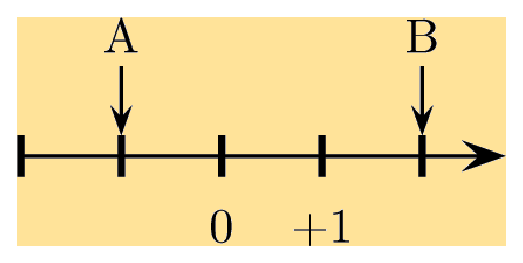
\includegraphics[width=2.6cm]{axeAB} \end{center}

      \begin{ChoixQCM}{4}
      \item $-1$
      \item $-2$
      \item positive
      \item négative
      \end{ChoixQCM}
\begin{corrige}
     \reponseQCM{ad} 
   \end{corrige}
    \end{exercice}
    
    
     \begin{exercice}
      Sur la droite précédente, l'abscisse de $B$ est \ldots
      \begin{ChoixQCM}{4}
      \item l'opposé de celle de $A$
      \item la valeur absolue de $-2$
      \item la valeur absolue de celle de $A$
      \item positive
      \end{ChoixQCM}
\begin{corrige}
     \reponseQCM{bd} 
   \end{corrige}
    \end{exercice}
    

    \begin{exercice}
      L'abscisse de $B$ est \ldots \hspace{0.4em} l'abscisse de $A$. 
      
\vspace{-2em}
\begin{center} 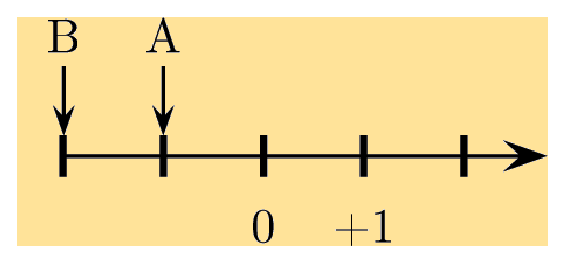
\includegraphics[width=2.6cm]{axeBA} \end{center}

      \begin{ChoixQCM}{4}
      \item plus grande que
      \item plus petite que
      \item $>$
      \item $<$
      \end{ChoixQCM}
\begin{corrige}
     \reponseQCM{bd} 
   \end{corrige}
    \end{exercice}
    
 
     \begin{exercice}
      $-3$ est \ldots 3
      \begin{ChoixQCM}{4}
      \item plus grand que
      \item plus petit que
      \item la valeur absolue de
      \item l'opposé de de
      \end{ChoixQCM}
\begin{corrige}
     \reponseQCM{bd} 
   \end{corrige}
    \end{exercice}
 \end{GroupeQCM}
\end{QCM}
 
 
\begin{QCM}
  \begin{GroupeQCM}   
    \begin{exercice}
      $-5$ \ldots $-7$
      \begin{ChoixQCM}{4}
      \item $>$
      \item $<$
      \end{ChoixQCM}
\begin{corrige}
     \reponseQCM{a}
   \end{corrige}
    \end{exercice}
    

    
    \begin{exercice}
      $-30$ \ldots $-35$
      \begin{ChoixQCM}{4}
      \item $>$
      \item $<$
      \end{ChoixQCM}
\begin{corrige}
     \reponseQCM{a}
   \end{corrige}
    \end{exercice}
    \begin{exercice}
      $-1,95$ \ldots $-1,94$
      \begin{ChoixQCM}{4}
      \item $>$
      \item $<$
      \end{ChoixQCM}
\begin{corrige}
     \reponseQCM{b}
   \end{corrige}
    \end{exercice}
    
    
    \begin{exercice}
      $-2,04$ \ldots $-2,048$
      \begin{ChoixQCM}{4}
      \item $>$
      \item $<$
      \end{ChoixQCM}
\begin{corrige}
     \reponseQCM{a}
   \end{corrige}
    \end{exercice} 

\end{GroupeQCM}
\end{QCM}

  
